% % % % % % % % % % % % % % % % % % % % % % % % % % % % % % % % % % % % % % % %
%
%
\chapter{Derivations of the Governing Equations}
%
%
%
      The following chapter discusses the derivation of the continuity,
      momentum, total energy,  mechanical (kinetic) energy, thermo (internal)
      energy and enthalpy equation by using a small volume element d$V$. The
      equations are derived completely while using the Cartesian coordinate
      system. A summary of all discussed equations is given on page
      \pageref{SummationOfEquations}. The structure of this chapter is (mainly)
      as follows:
%
%
\begin{itemize}
 \item Express the phenomena that act on the volume element using finite differences,
 \item Transform the finite difference equation to a partial differential equation,
 \item Manipulate the equation to get the conserved Cartesian formulation,
 \item Transform the Cartesian into the vector notation,
 \item Perform a proof to demonstrate that the vector notation results in the Cartesian form,
 \item Transform the equation into the integral and non-conserved form.
\end{itemize}
%
%

	The primary references that were used in this chapter are
    \cite{  Bird, Versteeg, JasakPhD, Ferziger, Rappaz,  Schwarze, ProgrammersGuide}
    and \cite{Moukalled15}.
%
%
%
%
%
\section{The Continuity Equation}
%
%
	In the following section the derivation of the continuity equation is
    presented. The equation itself describes the mass balance of an arbitrary
    volume element d$V$.

	Consider the mass flow through a small control volume element d$V$, c.f.
    figure \ref{figure::massFigure}, while using the constrain that mass is
    not transformed into energy or vice versa, a mass balance has to be
    fulfilled for the volume element. That means, that the mass flow that enters
    and leaves the volume element through its surfaces has to be equal if the
    mass inside the control volume does not change by means of compression or
    expansion --- this is also named as \textit{rate of mass accumulation}.
    Considering a small control volume d$V$, we can say:
%
%
\begin{equation}
\left[
 \begin{matrix}
  \rmm{rate~of~mass}\\
  \rmm{accumulation}
 \end{matrix}
\right]
=
\left[
 \begin{matrix}
  \rmm{rate~of~mass}\\
  \rmm{entering~the~volume}
 \end{matrix}
\right]
-
\left[
 \begin{matrix}
  \rmm{rate~of~mass}\\
  \rmm{leaving~the~volume}
 \end{matrix}
\right].
\label{equation::massWord}
\end{equation}
%
%
	To keep clearance, we will now focus on figure \ref{figure::massFigure}.
    It is obvious that the quantity \texttt{mass} is transported through the
    surface by the velocity. This transport phenomenon is called convection or
    sometimes named advection. In literature we can find the different meaning
    of convection and advection as follows:
%
%
\begin{itemize}
 \item Advection: Transport of mass, momentum, energy, etc. based on the fluid
       flow (flux) without diffusion effects.
 \item Convection: Transport of any property based on fluxes and diffusion.
\end{itemize}
%
%
    However, personally I heard that convection and advection represents
    always the transport of the quantity of interest based on the fluxes,
    while the nomenclature of convection always if we are talking about the
    momentum equation (e.g. the source of fluxes) while other quantities are
    advected with the fluxes.

	The transport of mass happens in all three space directions $x$ ($u_x$),
    $y$ ($u_y$), and $z$ ($u_z$). Additionally, mass can change inside the
    control element d$V$ which is related to compression or expansion
    phenomenon. Thus, the density of the fluid inside the volume must change.
%
%
%
%
\begin{figure}[!b]
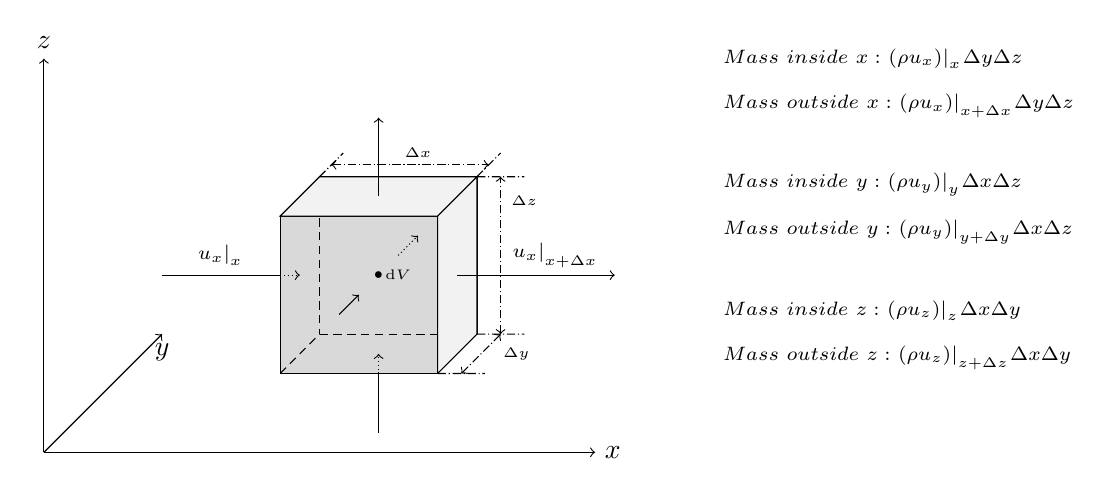
\begin{tikzpicture}
% Koordinatensystem
\draw[->] (0,0) -- (7,0) node[right] {$x$} coordinate(x axis);
\draw[->] (0,0) -- (0,5) node[above] {$z$} coordinate(z axis);
\draw[->] (0,0) -- (1.5,1.5) node[below] {$y$} coordinate(y axis);

% Quader
\draw [fill=gray!30] (3,1) -- (5,1) -- (5,3) -- (3,3) -- (3,1) ;

\draw [densely dashed] (3.5,1.5) -- (5.5,1.5);
\draw [] (5.5,1.5) -- (5.5,3.5) -- (3.5,3.5);
\draw [densely dashed] (3.5,3.5) -- (3.5,1.5);

\draw  [densely dashed] (3,1) -- (3.5,1.5);
\draw  [fill=gray!10] (5,1) -- (5.5,1.5) -- (5.5,3.5) -- (5,3) -- (5,1);
\draw  [fill=gray!10] (5,3) -- (5.5,3.5) --  (3.5,3.5) -- (3,3) -- (5,3);

%\draw (3,1) -- (3.5,3.5);
%\draw (3,3) -- (3.5,1.5);

% Pfeile
% rechts nach links
\draw [densely dotted, ->] (3,2.25) -- (3.25,2.25);
\draw [] (1.5,2.25) -- (3,2.25);
\draw [->] (5.25,2.25) -- (7.25,2.25);

% unten nach oben
\draw [] (4.25,0.25) -- (4.25,1);
\draw [densely dotted, ->] (4.25,1) -- (4.25,1.25);
\draw [->] (4.25,3.25) -- (4.25,4.25);

% vorn nach hinten
\draw [densely dotted, ->] (4.5,2.5) -- (4.75,2.75);
\draw [->] (3.75,1.75) -- (4,2);

% Punkte für Gleichungen
\node at (2.25,2.5) {\scriptsize $ u_x|_{_x}$};
\node at (6.5,2.5) {\scriptsize $ u_x|_{_{x+\Delta x}}$};

%\node at (4.5,0.5) {\scriptsize $ u_y|_{_y}$};
%\node at (4.5,4.2) {\scriptsize $ u_y|_{_{y+\Delta y}}$};

%\node at (4.5,2.75) {\scriptsize $ u_z|_{_x}$};
% \node at (4,1.75) {\scriptsize $ u_z|_{_{z+\Delta z}}$};

% Linien für dx dy dz
\draw [densely dashdotted] (5,1) -- (5.6,1)
	 (5.5,1.5) -- (6.1,1.5)
	 (5.5,3.5) -- (6.1, 3.5)
	 (3.5,3.5) -- (3.8,3.8)
	 (5.5,3.5) -- (5.8,3.8);

\draw [<->,densely dashdotted] (5.3,1) -- (5.8,1.5);
\node at (6,1.25) {\tiny $\Delta y$};

\draw [<->,densely dashdotted] (5.8,1.5) -- (5.8,3.5);
\node at (6.1,3.2) {\tiny $\Delta z$};

\draw [<->,densely dashdotted] (3.65,3.65) -- (5.65,3.65);
\node at (4.75,3.8) {\tiny $\Delta x$};

% Volumenpunkt
\node at (4.25,2.25) {\tiny $\bullet$};
\node at (4.5,2.25) {\tiny d$V$};


\node at (8.5,5) [right] {\scriptsize $ \rmm{Mass~inside~x:~} (\rho u_x)|_{_x} \Delta y \Delta z $};
\node at (8.5,4.4) [right] {\scriptsize $ \rmm{Mass~outside~x:~} (\rho u_x)|_{_{x+\Delta x}} \Delta y \Delta z $};

\node at (8.5,3.4) [right] {\scriptsize $ \rmm{Mass~inside~y:~} (\rho u_y)|_{_y} \Delta x \Delta z $};
\node at (8.5,2.8) [right] {\scriptsize $ \rmm{Mass~outside~y:~} (\rho u_y)|_{_{y+\Delta y}} \Delta x \Delta z $};

\node at (8.5,1.8) [right] {\scriptsize $ \rmm{Mass~inside~z:~} (\rho u_z)|_{_z} \Delta x \Delta y $};
\node at (8.5,1.2) [right] {\scriptsize $ \rmm{Mass~outside~z:~} (\rho u_z)|_{_{z+\Delta z}} \Delta x \Delta y $};

\end{tikzpicture}
\caption{Mass balance in a small volume element d$V$.}
\label{figure::massFigure}
\end{figure}
%
%
%
%

	Analysing figure \ref{figure::massFigure} in more detail, we observe that
    the velocity vectors are aligned normal to the surface faces. The rate of
    mass that enters or leaves the volume element through the surface is called
    mass flux and is simply the density multiplied by the velocity with respect
    to the face area.

	For the derivation of the mass conservation equation we have to build the
    balance of the surface fluxes at all faces of the control volume d$V$.
    In other words, everything that is going inside has to go out, if we
    assume that there is no mass accumulation inside the volume
    (assumption: incompressible). The single terms that describe the fluxes
    at the surfaces are given on the right side in figure \ref{figure::massFigure}.

	Considering a compressible fluid, the rate of mass change inside the
    control volume d$V$ is related to the density $\rho$ and will only
    decrease or increase with respect to the time. It is worth to mention that
    the quantity is defined to be \textbf{mass per unit volume}.
    Therefore, we can write the rate of change of the density as:
%
%
\begin{equation}
 \text{Time Accumulation} = \frac{\Delta \rho}{\Delta t}~.
 \label{EQUATION::densityTime}
\end{equation}
%
%
	Rewriting equation (\ref{equation::massWord}) by using the mathematical
    expressions given in figure \ref{figure::massFigure} and equation
    (\ref{EQUATION::densityTime}), it follows:
%
%
\begin{align*}
\frac{\Delta \rho}{\Delta t} \Delta x \Delta y \Delta z
&=
  \left((\rho u_x)|_{_x} - (\rho u_x)|_{_{x+\Delta x}}\right) \Delta y \Delta z \\
&+
  \left((\rho u_y)|_{_y} - (\rho u_y)|_{_{y+\Delta y}}\right) \Delta x \Delta z \\
&+
  \left((\rho u_z)|_{_z} - (\rho u_z)|_{_{z+\Delta z}}\right) \Delta x \Delta y~.
  \numberthis
\end{align*}
%
%
	Dividing the equation by the volume $\Delta V = \Delta x \Delta y \Delta z$,
    we end up with the following:
%
%
\begin{align*}
 \frac{\Delta \rho}{\Delta t}
&=
  \frac{(\rho u_x)|_{_x} - (\rho u_x)|_{_{x+\Delta x}}}{\Delta x} \\
&+
  \frac{(\rho u_y)|_{_y} - (\rho u_y)|_{_{y+\Delta y}}}{\Delta y} \\
&+
  \frac{(\rho u_z)|_{_z} - (\rho u_z)|_{_{z+\Delta z}}}{\Delta z}
  \numberthis ~.
  \label{EQUATION::ab}
\end{align*}
%
%
	Introducing the assumption of an infinitesimal small volume element ---
    which means that we decrease the distance between the corners of the
    volume and therefore, $\Delta$ goes to the limit to become zero:
%
%
\begin{equation}
 \frac{\Delta}{\Delta x}
    ~ ~ \longrightarrow
    ~ ~ \lim_{\Delta x \to 0}{\frac{\Delta}{\Delta x}}
    = \frac{\partial}{\partial x}~,
 \label{EQUATION::infty}
\end{equation}
%
%
	and also an infinitesimally small time range:
%
%
\begin{equation}
 \frac{\Delta}{\Delta t}
    ~ ~ \longrightarrow
    ~ ~ \lim_{\Delta t \to 0}{\frac{\Delta}{\Delta t}}
    = \frac{\partial}{\partial t} ~,
  \label{EQUATION::inftyTime}
\end{equation}
%
%
	we can transform the finite difference equation to a partial differential
    equation. For that, we have to apply equation (\ref{EQUATION::infty}) and
    (\ref{EQUATION::inftyTime}) to (\ref{EQUATION::ab}). It follows:
%
%
\begin{equation}
 \frac{(\rho u_x)|_{_x} - (\rho u_x)|_{_{x+\Delta x}}}{\Delta x} = \frac{-\Delta (\rho u_x)}{\Delta x}
\longrightarrow
-\frac{\partial}{\partial x} (\rho u_x)~,
\end{equation}
\begin{equation}
\frac{(\rho u_y)|_{_y} - (\rho u_y)|_{_{y+\Delta y}}}{\Delta y} = \frac{-\Delta (\rho u_y)}{\Delta y}
\longrightarrow
-\frac{\partial}{\partial y} (\rho u_y) ~,
\end{equation}
\begin{equation}
\frac{(\rho u_z)|_{_z} - (\rho u_x)|_{_{z+\Delta z}}}{\Delta z} = \frac{-\Delta (\rho u_z)}{\Delta z}
\longrightarrow
-\frac{\partial}{\partial z} (\rho u_z) ~,
\end{equation}
\begin{equation}
  \frac{\Delta \rho}{\Delta t} \to \frac{\partial \rho}{\partial t} ~,
\end{equation}
%
%
%
%
	and therefore, the general mass conservation (continuity) equation is
    given by:
%
%
\begin{equation}
\boxed{
 \frac{\partial \rho}{\partial t} =
 - \left(
      \frac{\partial}{\partial x} (\rho u_x)
    + \frac{\partial}{\partial y} (\rho u_y)
    + \frac{\partial}{\partial z} (\rho u_z)
   \right)
   } ~.
\end{equation}
%
%
	While using the Nabla-Operator $\nabla$ and the velocity vector
    \textbf{U}, the equation can be rewritten in vector notation:
%
%
\begin{equation}
\boxed{
 \frac{\partial \rho}{\partial t} =
 -   \nabla \bullet \left(\rho \textbf{U}\right)
   } ~.
   \label{EQUATION::massCompressible}
\end{equation}
%
%
	However, if we focus on incompressible fluids, we can assume that the
    density is constant and therefore, the quantity $\rho$ can be taken out of
    the derivatives and the whole equation can be divide by the density $\rho$.
    It is obvious that the time derivative will vanish due to the fact that
    the density is a constant. In other words, there is no accumulation of
    mass during the time in the volume element.
    One may also explain it in the following way: If we assume a constant
    density, there is no expansion or compression phenomena and therefore,
    the time derivative become zero. Hence, only the mass flux that enters
    and/or leaves the volume element at its surface has to be taken into account.

	For incompressible cases, the density for the fluid is constant and thus,
    we can simplify the mass conservation equation to:
%
%
\begin{equation}
 \boxed{  \nabla \bullet \textbf{U} = 0} ~.
 \label{EQUATION::massIncompressible}
\end{equation}
%
%
	In case of the incompressible mass conservation equation, it is evident
    that the vector notation results in the Cartesian form again. Thus,
    the transformation is not demonstrated here. If one wants to recheck it,
    just use equation (\ref{EQUATION::divVector}).

	\textbf{Remark}: In many cases incompressibility means that there is no
    expansion and/or compression phenomena. However, the fluid density can
    still be temperature depended and therefore, the quantity is not a
    constant. In such cases we have to be careful which mass conservation
    equation is used in the computational calculation. Either the
    incompressible or the compressible one.

	In general, if the density is not a constant value, we are not allowed to
    use the simplified mass conservation equation
    (\ref{EQUATION::massIncompressible}) due to the fact, that non-constant
    quantities are not allowed to be taken out of the derivatives. However,
    if the density change is very small, we can use the incompressible mass
    conservation equation with limitations. The reason for that is based
    on numerics and the interaction with the momentum conservation equation.

%
%
\subsection{Integral Form of the Conserved Continuity Equation}
%
%
	For the completeness, the integral form of the mass conservation equation
    will be given now. While using the Gauss theorem
    (\ref{EQUATION::gausstheorem}), we can transform the divergence term
    (that acts on the volume) to a surface integral. The accumulation of
    density in the element is a simple volume integral. Furthermore, the
    volume element d$V$ itself does not change its shape with respect to
    the time (fixed finite volume - static mesh). Thus, we end up with:
%
%

	Compressible:
%
%
\begin{equation}
 \boxed{
 \frac{\partial}{\partial t} \int \rho \mathrm{d}V=
 -   \oint \rho \textbf{U} \cdot \textbf{n} \mathrm{d}S
   } ~.
\end{equation}
%
%

	Incompressible:
%
%
\begin{equation}
 \boxed{
    \oint \textbf{U} \cdot \textbf{n} \mathrm{d}S = 0
   } ~.
\end{equation}
%
%
	The surface integral means nothing more than taking the balance of
    the fluxes on the surfaces of the volume element; what is going in
    and out. Depending on the shape of the volume, we have to evaluate
    more or less faces. The integral form of the continuity equation leads
    to the so called finite volume method (FVM). This method is conservative
    and we can apply this method to arbitrary volumes such as hexahedral,
    tetrahedral, prisms, wedges and so on. This advantage made this method
    popular and flexible. However, it is worth to mention that the shape
    of the volumes influences the numerical stability and the calculation
    precision in general.
%
%
%
%
%
\subsubsection{\OF}
%
%
	In \OF we are using the equations (integral one) above to calculate
    the fluxes at the faces of each numerical cell. The flux field is
    named \texttt{phi} and is created by including one of the two header
    files in each solver:
%
%
\begin{itemize}
 \item createPhi.H
 \item compressibleCreatePhi.H
\end{itemize}
%
%
	Due to the fact that we store the density and the velocity at the
    cell center, we need to interpolate these values to the face centers.
    This calculation is done by calling the function
    \texttt{interpolate(rho*U) \& mesh.Sf()}. As we can see, this will
    simply calculate the product of the density and the velocity vector
    at each cell center and interpolate the result to the face center by
    including the corresponding neighbor cell information. To get the fluxes,
    the known face values are then multiplied by the magnitude of the surface
    normal vector (\texttt{Sf()}). The calculation is an inner product
    operation of two vectors which is denoted by the ampersand sign
    \texttt{\&} in \OF.
%
%
%
%
%
\subsection{Continuity Equation and the Total Derivative}
%
%
	In the first chapter, while introducing basic mathematical operation,
    we already mentioned the total derivative. After knowing the continuity
    equation, we can investigate into it in more detail.

	Using the total derivative formulation (\ref{EQUATION::totalDerivative}),
    we are able to rewrite the continuity equation
    (\ref{EQUATION::massCompressible}) by applying the product rule
    (\ref{EQUATION::productRuleVS}) to the divergence term:
%
%
\begin{equation}
  \nabla \bullet \left(\rho \textbf{U}\right)
=
  \textbf{U} \bullet \nabla \rho + \rho \nabla \bullet \textbf{U} ~.
\end{equation}
%
%
	Substituting this expression into equation
    (\ref{EQUATION::massCompressible}), we get:
%
%
\begin{equation}
 \frac{\partial \rho}{\partial t}
 =
 -\textbf{U} \bullet \nabla \rho - \rho \nabla \bullet \textbf{U} ~.
\end{equation}
%
%
	Finally, we put all terms to the LHS:
%
%
\begin{equation}
 \underbrace{\frac{\partial \rho}{\partial t}
+
 \textbf{U} \bullet \nabla \rho}_{\mathrm{Total~derivative}}
+
 \rho \nabla \bullet \textbf{U}
 =
0 ~.
\end{equation}
%
%
	The result is:
%
%
\begin{equation}
 \frac{\mathrm{D} \rho}{\mathrm{D} t}
+
 \rho \nabla \bullet \textbf{U}
 =
0 ~.
\end{equation}
%
%
	This equation is not common but could be found for example in
    \cite{Anderson}.


%==============================================================================
